\subsection{Hệ thông gợi ý (Recomender System)}
Recommender System (RS) hay Reacommendation system là một mảng của Infomation filtering system dùng để đưa ra những gợi ý phù hợp nhất cho người dùng. Recommender system được ứng dụng trên nhiều lĩnh vực như phim, nhạc, tin tức, sách,... Ngoài ra còn ứng dụng trong hệ thống giới thiệu cho các chuyên gia, cộng tác viên, nhà hàng, dịch vụ tài chính, mạng xã hội.
Một ví dụ điển hình đối với trang thương mại điện tử Amazone đã làm như sau:
\begin{itemize}
    \item Quan tâm đến việc khách hàng yêu thích những sản phẩm dựa vào dữ liệu quá khứ của họ như điểm đánh giá trên từng sản phẩm, thời gian duyệt trên từng sản phẩm, số lần click vào sản phẩm...
    \item Từ đó có thể dự đoán được người dùng có thể sẽ thích sản phẩm nào khác và đưa ra gợi ý phù hợp cho họ.
\end{itemize}

Trong RS chỉ có hai đối tượng được hướng tới đó là người dùng và nội dung. Cho nên việc phân loại hệ thống cũng được dựa trên hai đối tượng trên.

\textbf{Hệ thống gợi ý dựa trên nội dung (Content based recommender system)} Hệ thống sẽ quan tâm đến nội dung hiện tại và sau đó  đưa ra gợi ý cho người dùng các mục tin tương tự. Ví dụ khi truy cập vào youtube.com thì youtube dưa ra gợi ý video những thể loại mà người dùng thường xuyên xem dựa vào lịch sử xem video của người dùng. Tuy nhiên điểm hay của youtube là khi user đang xem một video bất kì với chủ đề mới mà trước đó chưa xem thì việc đưa ra gợi ý không phải dựa vào lịch sử mà gợi ý dựa vào nội dung video hiện tại mà user đang xem.

\textbf{Hệ thống gợi ý dựa trên user (Collaborative filltering recommender systems} hệ thống phân tích hành vi của user để đưa ra sự tương đồng sở thích giữa các user với nhau để đưa ra gợi ý.

\begin{figure}[h]
\centering
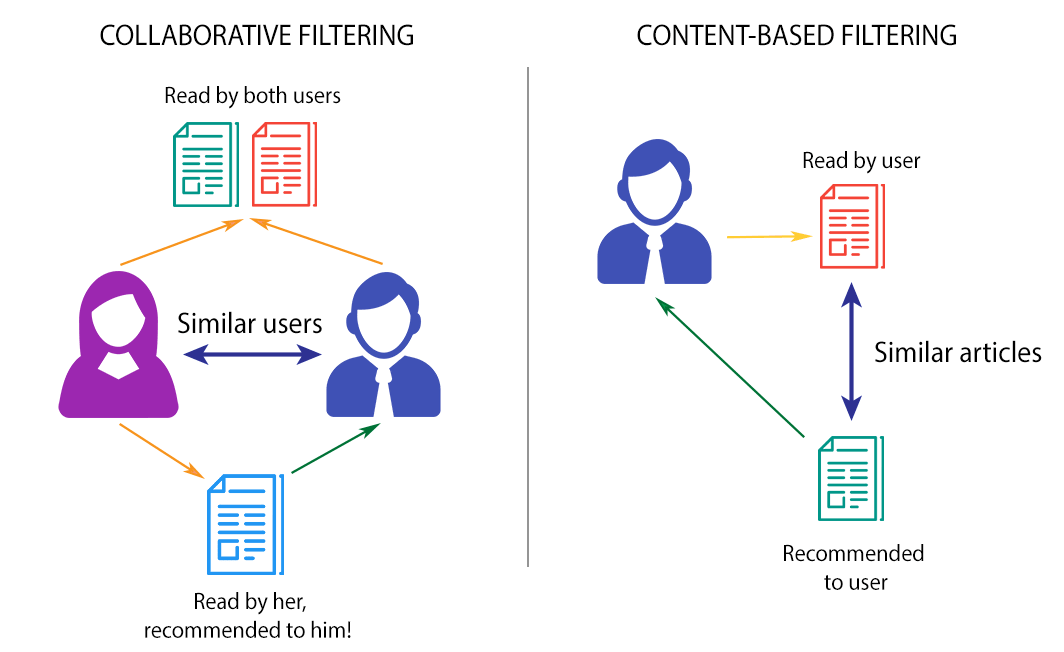
\includegraphics[width=13cm]{image/Collaborative-Filtering-min.png}
\caption{Hệ thống gợi ý dựa trên nội dung và dựa trên user}
\end{figure}

\textbf{Hybrid recommender system} là việc kết hợp hai hệ thống trên nhằm đưa ra kết quả tốt hơn. Phương pháp này thực hiện bằng cách đưa các dự đoán dựa trên nội dung và hợp tác độc lập với sau và sau đó kết hợp chúng lại. Hoặc bằng cách khác là đưa ra mô hình thống nhất các phương pháp tiếp cận thành một mô hình. Hybrid system đưa ra khuyến nghị chính xác hơn các phương pháp thuần túy.  

\textbf{Chuẩn bị dữ liệu}
Đối với đề tài này dữ liệu được thu thập từ ba nguồn dữ liệu phản hồi từ mail sinh viên, dữ liệu tương tác của sinh viên từ hệ thống, và cuối cùng là dữ liệu từ nguồn khác như điểm sinh viên, số ngày công tác xã hội,...

Những bài viết, hoạt động được phân loại trước ví dụ bài đăng về tuyển dụng, hoạt động đoàn thanh niên, hoạt động công tác xã hội,... Dựa trên những phân loại về bài đăng hệ thống sẽ tìm sinh viên phù hợp với sinh viên đó sau đó gửi mail cho sinh viên hoặc đưa những mục tin phù hợp với sinh viên khi sinh viên truy cập vào hệ thống. 

Ma trận dữ liệu khi thu thập từ sinh viên là ma trận thưa, cho nên cần chuẩn hóa dữ liệu trước khi chạy giải thuật. Việc chuẩn hóa dưới đây là một ví dụ mẫu, vì trên thực tế có nhiều cách khác nhau để thực hiện việc chuẩn hóa. Ví dụ trong trường hợp đơn giản  doanh nghiệp cần tuyển dụng sinh viên năm hai trở lên và có điểm trung bình trên 5.0 thì việc chuẩn hóa dữ liệu không nhất thiết là số năm học tại trường là 1, 2, 3. Hay lấy điểm sinh viên với phổ điểm từ 0 đến 10 mà chỉ cần các giá trị 0 1 là có thể xác định được độ phù hợp của sinh viên đó đối với yêu cầu tuyển dụng.

\begin{figure}[h]
\centering
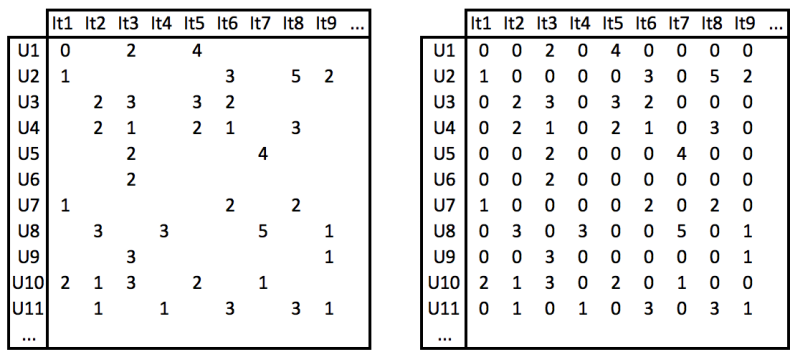
\includegraphics[width=13cm]{image/data-normalization.png}
\caption{Ví dụ cấu trúc ma trận dữ liệu trước và sau khi chuẩn hóa}
\end{figure}

Việc đưa ra gợi ý một cách chính xác thì cần có nhiều tiêu chí đánh giá khác nhau như điểm trung bình, số ngày công tác xã hội, sở thích, các hoạt động đã tham gia,... Và những tiêu chí này cần được sắp xếp thứ tự ưu tiên khi xét một hoạt động hay một bài đăng trong hệ thống. Ví dụ những bài đăng về tuyển dụng của doanh nghiệp sẽ có tiêu chí đánh giá khác những bài đăng về các hoạt động công tác xã hội. Cho nên việc thống nhất và chọn mô hình phù hợp với bài toán là điều khó khăn trong giai đoạn đề cương.

\subsection{Cơ sở dữ liệu (Database)}
\subsubsection{Hệ cơ sở dữ liệu quan hệ (RDBMS)}
\textbf{Khái niệm:}
\par
RDBMS - Relational Database Management System - là hệ quản trị cơ sỡ dữ liệu quan hệ. RDBMS là cơ sở cho SQL, và cho tất cả các hệ thống cơ sở dữ liệu hiện đại như MS SQL Server, IBM DB2, Oracle, MySQL và Microsoft Access.
\par
\textbf{Bảng:}
\par
Dữ liệu trong một RDBMS được lưu trữ trong các đối tượng cơ sở dữ liệu được gọi là các bảng (table) . Bảng này về cơ bản là một bộ sưu tập các mục nhập dữ liệu có liên quan và nó bao gồm nhiều cột và hàng.
Bảng là hình thức lưu trữ dữ liệu phổ biến và đơn giản nhất trong một cơ sở dữ liệu quan hệ. Chương trình sau đây là một ví dụ về một bảng KHACH\_HANG

\begin{table}[h]
    \centering
    \begin{tabular}{ |c|l|r|l|r| } 
    \hline
    ID & TEN & TUOI & DIA\_CHI & LUONG \\ 
    \hline
    1 & Nam & 32 & Ha Noi & 2000.00 \\
    \hline
    2 & Dung & 25 & Ho Chi Minh & 1500.00 \\
    \hline
    3 & Vinh & 23 & Ha Noi & 2000.00 \\
    \hline
    \end{tabular}
    \caption{Ví dụ về bảng dữ liệu}
    \label{tab:table_data}
\end{table}



\textbf{Trường:}
\par
Mỗi bảng được chia thành các thực thể nhỏ gọi là các trường (Field). Các trường trong bảng KHACH\_HANG bao gồm ID, TEN, TUOI, DIA\_CHI VÀ LUONG.
Trường là một cột trong một bảng được thiết kế để lưu trữ thông tin cụ thể về mỗi bản ghi trong bảng.
Ví dụ: một cột trong bảng KHÁCH HÀNG là DIA\_CHI, mô tả vị trí và sẽ như dưới đây

\begin{table}[h]
    \centering
    \begin{tabular}{ |l| } 
     \hline
     DIA\_CHI \\
     \hline
     Ha Noi \\
     \hline
     Ho Chi Minh \\
     \hline
     Ha Noi \\
     \hline
    \end{tabular}
    \caption{Ví dụ về một trường trong bảng dữ liệu}
    \label{tab:column_data}
\end{table}

\textbf{Bản ghi hoặc hàng:}
\par
Một bản ghi (record) cũng được gọi là một hàng (row) dữ liệu là từng mục riêng lẻ tồn tại trong một bảng. Ví dụ: có 3 bản ghi trong bảng KHACH\_HANG trên. Sau đây là một hàng dữ liệu hoặc một bản ghi trong bảng, ví dụ bảng \ref{tab:row_data}

\begin{table}[h!]
    \centering
    \begin{tabular}{ |c|l|r|l|r| } 
     \hline
     1 & Nam & 32 & Ha Noi & 2000.00 \\
     \hline
    \end{tabular}
    \caption{Ví dụ một bản ghi trong bảng dữ liệu}
    \label{tab:row_data}
\end{table}

\textbf{Ràng buộc:}
\par
Ràng buộc (Constraint) là các quy tắc được thi hành trên các cột dữ liệu trên một bảng. Chúng được sử dụng để giới hạn loại dữ liệu có thể insert vào một bảng. Điều này đảm bảo tính chính xác và độ tin cậy của dữ liệu trong cơ sở dữ liệu.
\par
Constraint có thể là cấp độ cột hoặc cấp độ bảng. Các ràng buộc cấp độ cột chỉ được áp dụng cho một cột trong khi các ràng buộc mức bảng được áp dụng cho toàn bộ bảng.
\par
Sau đây là một số các ràng buộc phổ biến nhất được sử dụng trong SQL:

\begin{table}[h]
    \centering
    \begin{tabular}{|l|l|} 
     \hline
     \textcolor{green}{NOT NULL} & Đảm bảo rằng một field không thể có giá trị NULL\\
     \hline
     \textcolor{green}{DEFAULT} & Cung cấp một giá trị mặc định cho một field khi không có gì được chỉ định \\
     \hline
     \textcolor{green}{UNIQUE} & Đảm bảo rằng tất cả các giá trị trong một field  khác nhau\\
     \hline
     \textcolor{green}{PRIMARY Key} & Xác định mỗi record là duy nhất trong một bảng cơ sở dữ liệu\\
     \hline
     \textcolor{green}{FOREIGN Key} & Xác định một record là duy nhất trong bất kỳ bảng cơ sở dữ liệu khác \\
     \hline
     \textcolor{green}{CHECK} & CHECK constraint đảm bảo rằng tất cả các giá trị trong một cột thoả mãn một số điều kiện \\
     \hline
     \textcolor{green}{INDEX} & Dùng để tạo và lấy dữ liệu từ cơ sở dữ liệu rất nhanh\\
     \hline
    \end{tabular}
    \caption{Một số ràng buộc phổ biến trong SQL}
    \label{tab:contrain_data}
\end{table}

\textbf{Toàn vẹn dữ liệu:}
\par
Các loại sau đây của toàn vẹn dữ liệu tồn tại với mỗi RDBMS:
\begin{itemize}
    \item \textbf{Thực thể toàn vẹn} – Không có hàng trùng lặp trong một bảng.
    \item \textbf{Domain Integrity} -  Thực thi kiểm tra tính hợp lệ cho một cột nhất định bằng cách hạn chế kiểu, định dạng hoặc phạm vi giá trị.
    \item \textbf{Tính toàn vẹn tham chiếu} - Các hàng không thể bị xóa, được sử dụng bởi các bản ghi khác.
    \item \textbf{Tính toàn vẹn do người dùng định nghĩa} - Thực thi một số quy tắc kinh doanh cụ thể không rơi vào thực thể, miền hoặc toàn vẹn tham chiếu.
\end{itemize}
\textbf{Các hệ quản trị cơ sở dữ liệu:}
\par
Hiện nay, có rất nhiều RDBMS – hệ quản trị cơ sở dữ liệu phổ biến có sẵn để làm việc. Hướng dẫn này đưa ra một cái nhìn ngắn gọn về một số các RDBMS phổ biến nhất.
\begin{table}[h]
\centering
\begin{tabular}{|l|l|l|} 
 \hline
 RDBMS & Giới thiệu & Tính năng, đặc điểm \\
 \hline
 \multicolumn{1}{|p{2cm}|}{MySQL} & \multicolumn{1}{p{7cm}|}{MySQL là RDBMS SQL mã nguồn mở, MySQL hỗ trợ nhiều nền tảng khác nhau bao gồm MS.Windows, Linux, UNIX và Mac OS X. MySQL đi kèm với một máy chủ DB SQL rất nhanh, đa luồng, nhiều người dùng và mạnh mẽ.} & \multicolumn{1}{p{6cm}|}{Hiệu suất cao, Tính sẵn sàng cao, Khả năng mở rộng và Tính linh hoạt Chạy bất cứ điều gì, Hỗ trợ giao dịch mạnh mẽ, Điểm mạnh của Web và Data Warehouse, Bảo vệ dữ liệu mạnh mẽ, Phát triển ứng dụng toàn diện, Quản lý dễ dàng, nguồn mở và hỗ trợ 24/7, Tổng chi phí sở hữu thấp nhất.}\\
 \hline
 \multicolumn{1}{|p{2cm}|}{MS SQL Server} & \multicolumn{1}{p{7cm}|}{MS SQL Server là RDBMS được phát triển bởi MS.Inc Ngôn ngữ truy vấn chính: T-SQL, ANSI SQL} & \multicolumn{1}{p{6cm}|}{Hiệu năng cao, Tính sẵn sàng cao, Database mirroring, Database snapshots, Tích CLR, Service Broker, DDL triggers, Ranking, Row version-based isolation levels, Tích hợp XML, TRY…CATCH – xử lý ngoại lệ, Database Mail}\\
 \hline
 \multicolumn{1}{|p{2cm}|}{MS Access} & \multicolumn{1}{p{7cm}|}{Đây là một trong những sản phẩm phổ biến nhất của Microsoft. Microsoft Access là một phần mềm quản lý cơ sở dữ liệu cấp cơ sở. Cơ sở dữ liệu MS Access không chỉ là không tốn kém mà còn là một cơ sở dữ liệu mạnh mẽ cho các dự án quy mô nhỏ. MS Access sử dụng công cụ cơ sở dữ liệu Jet, sử dụng một ngôn ngữ cụ thể ngôn ngữ SQL (đôi khi được gọi là Jet SQL). MS Access đi kèm với phiên bản chuyên nghiệp của gói MS Office. MS Access có giao diện đồ họa trực quan sử dụng easyto.} & \multicolumn{1}{p{6cm}|}{Người dùng có thể tạo table, query, form, report, macro;Nhập và xuất dữ liệu sang nhiều định dạng (Excel, SQL Server, Oracle, ODBC …); Có định dạng Jet Database, điều này làm cho nó rất thuận tiện để phân phối toàn bộ ứng dụng cho người dùng khác,chấp nhận ngoại tuyến; MS Access cung cấp truy vấn tham số. MS Access là một cơ sở dữ liệu dựa trên máy chủ tập tin. Không giống như các RDBMS khách hàng, MS Access không thực hiện các trình khởi tạo cơ sở dữ liệu, các thủ tục lưu trữ hoặc đăng nhập giao dịch.
}\\
\hline
\end{tabular}
\end{table}

\begin{table}[h]
\centering
\begin{tabular}{|l|l|l|} 
\hline
 \multicolumn{1}{|p{2cm}|}{Oracle} & \multicolumn{1}{p{7cm}|}{Đây là RDBMS đa người dùng rất lớn. Oracle là RDBMS được phát triển bởi ‘Tổng công ty Oracle’. Oracle làm việc để quản lý một cơ sở dữ liệu thông tin giữa nhiều khách hàng yêu cầu và gửi dữ liệu trong mạng. Đây là một lựa chọn máy chủ cơ sở dữ liệu tuyệt vời cho khách hàng / máy tính. Oracle hỗ trợ tất cả các hệ điều hành chính cho cả khách hàng và máy chủ, bao gồm MSDOS, NetWare, UnixWare, OS / 2 và hầu hết các UNIX.} & \multicolumn{1}{p{6cm}|}{Truy cập đồng thời, Đọc tính nhất quán, Cơ chế khóa, Cơ sở dữ liệu Quiesce, Tính khả chuyển, Cơ sở dữ liệu tự quản lý, SQL*Plus, ASM, Scheduler, Quản lý Tài nguyên, Data Warehousing, Materialized views, Bitmap indexes, Table compression, Thực thi song song, Phân tích SQL, Data mining, Partitioning}\\
 
 \hline
\end{tabular}
\caption{Các hệ quản trị cơ sở dữ liệu thường gặp}
 \label{tab:dbms}
\end{table}

\newpage
\subsubsection{Hệ cơ sở dữ liệu phi quan hệ (Non-RDBMS)}
\par
Hệ cơ sở dữ liệu phi quan hệ là cơ sở dữ liệu không kết hợp mô hình table/key mà các RDBMS khác. Những loại cơ sở dữ liệu này đòi hỏi các kỹ thuật và quy trình xử lý dữ liệu để cung cấp các giải pháp cho các vấn đề dữ liệu lớn mà các công ty lớn gặp phải. Cơ sở dữ liệu phi quan hệ (Non-relational database) phổ biến nhất được gọi là NoSQL
\par
Hầu hết các hệ cơ sở dữ liệu phi quan hệ được kết hợp vào các trang Web lớn như Google, Yahoo!, Amazon, Facebook, ... Các trang web này đưa ra một loạt các ứng dụng mới mỗi ngày với hàng triệu và hàng triệu người dùng, vì vậy họ sẽ không thể xử lý các lưu lượng truy cập lớn với các giải pháp RDBMS hiện có. Do RDBMS không thể xử lý vấn đề, nên họ đã chuyển sang một loại DBMS mới có khả năng xử lý dữ liệu quy mô web theo cách phi quan hệ
\par
Một điều thú vị của NoSQL là khả năng mở rộng. NoSQL sử dụng hệ thống BASE (về cơ bản là có sẵn, softstate, nhất quán). Non-RDBMS từ bỏ dạng bảng của các hàng và cột cơ sở dữ liệu quan hệ sử dụng có lợi cho các khung chuyên dụng để lưu trữ dữ liệu, có thể được truy cập bằng các API truy vấn đặc biệt. Sự tồn lưu (Persistence) là một yếu tố quan trọng trong các cơ sở dữ liệu này. Để cho phép thông lượng nhanh với số lượng lớn dữ liệu, tuỳ chọn tốt nhất cho hiệu suất là "bộ nhớ trong", thay vì đọc và ghi từ ổ đĩa.
\par
Cơ sở dữ liệu quan hệ sử dụng hệ ACID, đảm bảo tính thống nhất của dữ liệu trong mọi tình huống quản lý dữ liệu nhưng rõ ràng mất nhiều thời gian hơn để xử lý vì tất cả các mối quan hệ đó và tính chất phân nhánh của nó. Tuy nhiên hệ thống BASE đã nới lỏng các yêu cầu về tính nhất quán để đạt được tính sẵn sàng và phân vùng tốt hơn để có khả năng mở rộng tốt hơn.
\par
\textbf{Các Non-RDBMS phổ biến}
\begin{enumerate}
    \item \textbf{Document database (CouchDB, MongoDB)}
    Dữ liệu thêm vào sẽ được lưu trữ dưới dạng cấu trúc JSON tự do hoặc document, ở đó dữ liệu có thể là bất kỳ dạng nào từ số nguyên đến chuỗi dữ liệu đến văn bản dạng tự do.
    \item \textbf{Key-value stores (Redis, Riak)}
    Các giá trị dạng tự do — từ các số nguyên hoặc chuỗi đơn giản đến các tài liệu JSON phức tạp — truy cập được trong cơ sở dữ liệu sử dụng các phím.
    \item \textbf{Wide column stores (HBase, Cassandra)}
    Dữ liệu được lưu trữ dạng cột thay vì theo hàng như trong hệ thống SQL thông thường. Bất kỳ số cột nào (và do đó có nhiều loại dữ liệu khác nhau) có thể được nhóm hoặc tổng hợp khi cần thiết cho các truy vấn hoặc chế độ xem dữ liệu.
    \item \textbf{Graph database (Neo4j)}
    Dữ liệu được biểu diễn dưới dạng mạng hoặc đồ thị các đối tượng và mối quan hệ của các đối tượng đó, với mỗi node trong biểu đồ là một đoạn dữ liệu dạng tự do.
\end{enumerate}
\subsubsection{So sánh Relational Database và Non-relational Database}
\begin{table}[h]
\centering
\begin{tabular}{|l|l|l|} 
 \hline
 Hạng mục & Relational & Non-relational \\
 \hline
 \multicolumn{1}{|p{2cm}|}{Kiểu dữ liệu} & \multicolumn{1}{p{6cm}|}{Khó lưu trữ kiểu dữ liệu phong phú} & \multicolumn{1}{p{7cm}|}{Có thể lưu trữ bất kỳ loại dữ liệu nào}\\
 \hline
 \multicolumn{1}{|p{2cm}|}{Nhân rộng} & \multicolumn{1}{p{6cm}|}{Khó để nhân rộng, chi phí không rẻ} & \multicolumn{1}{p{7cm}|}{Nhân rộng là tự động và trong suốt}\\
 \hline
 \multicolumn{1}{|p{2cm}|}{Chi phí} & \multicolumn{1}{p{6cm}|}{Chi phí xây dựng và bảo trì đắt} & \multicolumn{1}{p{7cm}|}{Khoảng 10\% chi phí so với Relational}\\
 \hline
 \multicolumn{1}{|p{2cm}|}{Hiển thị} & \multicolumn{1}{p{6cm}|}{Hiển thị dữ liệu trong bảng và hàng} & \multicolumn{1}{p{7cm}|}{Hiển thị dữ liệu dưới dạng JSON}\\
 \hline
 \multicolumn{1}{|p{2cm}|}{Truy vấn} & \multicolumn{1}{p{6cm}|}{Ngôn ngữ truy vấn có cấu trúc (SQL): làm cho khả năng tấn công là khả thi} & \multicolumn{1}{p{7cm}|}{Truy vấn đối tượng: trực quan, chuyển một tài liệu để giải thích những gì bạn đang truy vấn}\\
 \hline
 \multicolumn{1}{|p{2cm}|}{Đa nguồn gốc} & \multicolumn{1}{p{6cm}|}{Thực thi JOIN: thực hiện truy vấn trên nhiều bảng} & \multicolumn{1}{p{7cm}|}{Kiểu dữ liệu đa chiều: hỗ trợ mảng và thậm chí các tài liệu khác}\\
 \hline
 \multicolumn{1}{|p{2cm}|}{Kiểu nguyên tử (Atomic)} & \multicolumn{1}{p{6cm}|}{Hỗ trợ chuyển đổi: có thể chứa nhiều lệnh thực thi với một sự chuyển đổi và trả về nguyên vẹn toàn bộ nếu đó là một thực thi đơn lẻ} & \multicolumn{1}{p{7cm}|}{Không hỗ trợ, nhưng các thực thi đơn lẻ là các nguyên tử}\\
 \hline
 \multicolumn{1}{|p{2cm}|}{Lược đồ} & \multicolumn{1}{p{6cm}|}{Yêu cầu xác định bảng và cột trước khi lưu trữ. Mỗi hàng có cùng cột} & \multicolumn{1}{p{7cm}|}{Không có lược đồ, thả trong tài liệu. Hai tài liệu trong cùng một thu thập có thể có các trường khác nhau}\\
 \hline
 \end{tabular}
 \caption{So sánh cơ sở dữ liệu quan hệ và cơ sở dữ liệu phi quan hệ}
 \label{tab:compare_dbms}
\end{table}
\subsubsection{MongoDB}
\textbf{Tổng quan về MongoDB}
\par
Như đã được đề cập ở phần trên, MongoDB là một document database (non-RDBMS) với khả năng mở rộng và linh hoạt mà ta mong muốn với truy vấn và lập chỉ mục mà ta cần.
\begin{itemize}
    \item MongoDB lưu trữ dữ liệu trong các tài liệu linh hoạt, giống như JSON, có nghĩa là các trường có thể thay đổi từ tài liệu này sang tài liệu khác và cấu trúc dữ liệu có thể được thay đổi theo thời gian
    \item Mô hình tài liệu ánh xạ tới các đối tượng trong code, giúp dữ liệu được dễ dàng làm việc với nó.
    \item Truy vấn đặc biệt, lập chỉ mục và tổng hợp thời gian thực cung cấp cách mạnh mẽ để truy cập và phân tích dữ liệu
    \item MongoDB là một cơ sở dữ liệu phân tán ở cốt lõi của nó, vì vậy tính sẵn sàng cao, nhân rộng theo chiều ngang và phân phối vị trí được xây dựng và dễ sử dụng
    \item MongoDB là miễn phí và là nguồn mở.
\end{itemize}
\begin{figure}[h]
\centering
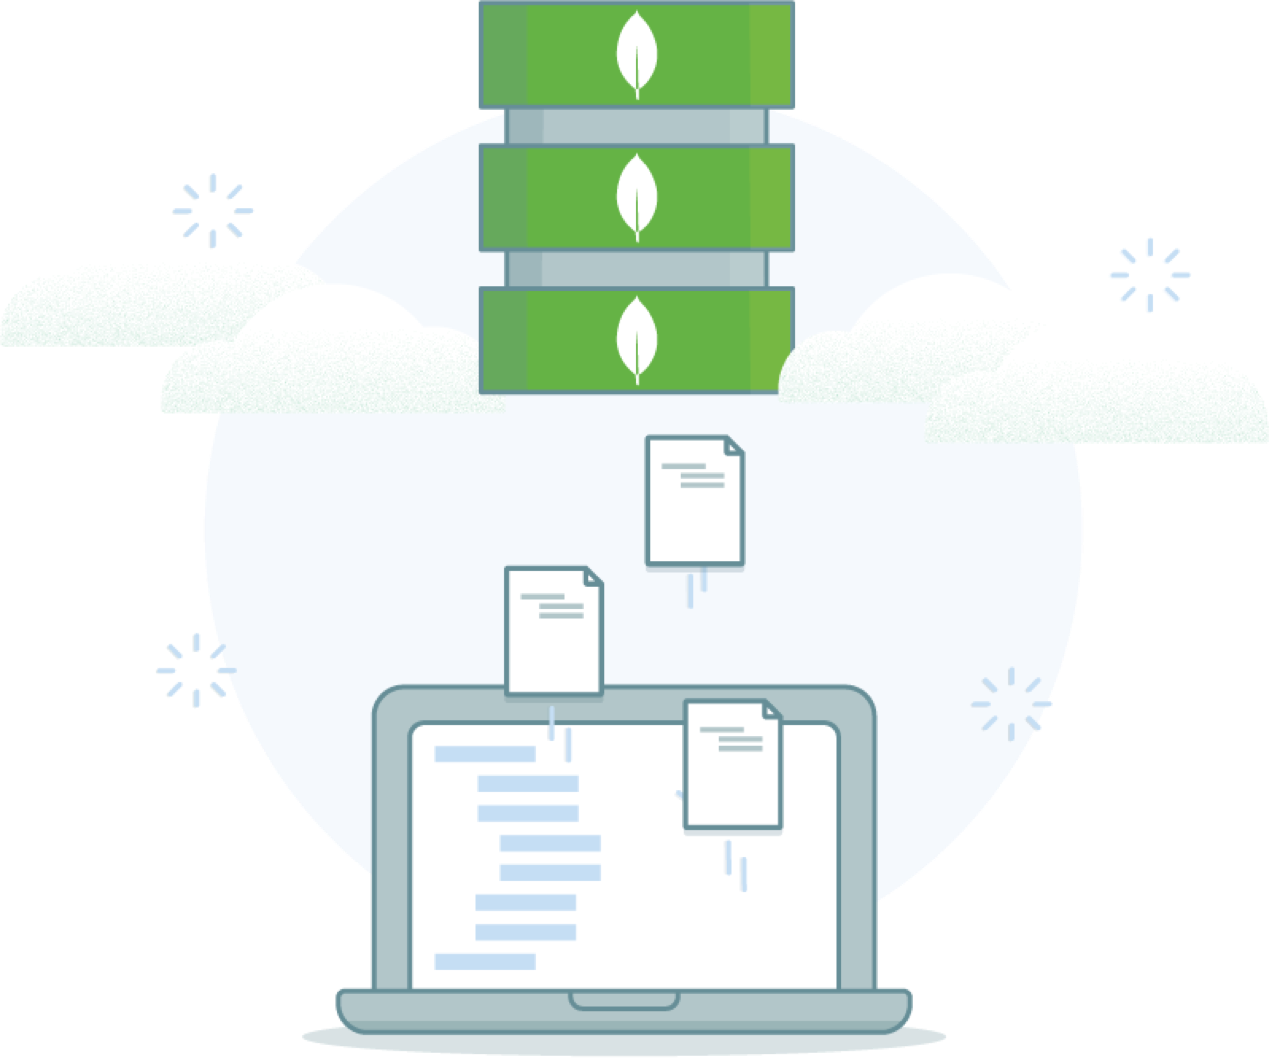
\includegraphics[width=10cm]{image/whats-mongodb-diagram.png}
\caption{MongoDB}
\label{fig:mongodb}
\end{figure}
\textbf{Sự lựa chọn MongoDB}
\par
Dựa vào các đối tượng mà đề tài hướng tới, hệ thống cần phải lưu một lượng dữ liệu lớn, các thuộc tính của dữ liệu có thể được thay đổi theo thời gian, chi phí xây dựng duy trì ổn định, thời gian truy vấn nhanh. Vì thế cho nên việc lựa chọn hệ cơ sở dữ liệu phi quan hệ là phù hợp cho hệ thống này.
\par
MongoDB là một hệ cơ sở dữ liệu phi quan hệ đáp ứng đẩy đủ nhu cầu dữ liệu của đề tài. MongoDB là miễn phí và là nguồn mở nên ta dễ dàng hiện thực ở phía Server bằng NodeJS. MongoDB lưu trữ dữ liệu dưới dạng JSON và hỗ trợ bất kỳ loại kiểu dữ liệu nào, việc tạo một Modal mới trở nên dễ dàng hơn. MongoDB hỗ trợ tốt trong việc nhân rộng dữ liệu, tính có sẵn cao là một sự cần thiết quan trọng cho đề tài.
\subsection{Phía server (Back-end)}
Back-end là thuật ngữ dùng trong lĩnh vực phát triển phần mềm gồm những thành phần xử lí thông tin từ phía server việc xử lí, phân tích dữ liệu và việc tương tác với hệ quản trị cơ sở dữ liệu (DBMS).
\subsubsection{Các công nghệ hiện tại}
Hiện nay với sự xuất hiện của nhiều ngôn ngữ lập trình khác nhau, kèm theo đó cũng có những công nghệ lập trình khác nhau dựa trên một ngôn ngữ cụ thể nào đó:

\textbf{Spring} là một Framework phát triển các ứng dụng Java được sử dụng bởi hàng triệu lập trình viên. Nó giúp tạo các ứng dụng có hiệu năng cao, dễ kiểm thử, sử dụng lại code…

Spring nhẹ và trong suốt (nhẹ: kích thước nhỏ, version cơ bản chỉ khoảng 2MB; trong suốt: hoạt động một cách trong suốt với lập trình viên)

Spring là một mã nguồn mở, được phát triển, chia sẻ và có cộng đồng người dùng rất lơn.

Spring Framework được xây dựng dựa trên 2 nguyên tắc design chính là: Dependency Injection và Aspect Oriented Programming.

Những tính năng core (cốt lõi) của Spring có thể được sử dụng để phát triển Java Desktop, ứng dụng mobile, Java Web. Mục tiêu chính của Spring là giúp phát triển các ứng dụng J2EE một cách dễ dàng hơn dựa trên mô hình sử dụng POJO (Plain Old Java Object)

\textbf{Django} là một web framework miễn phí mã nguồn mở được viết bằng Python. Django sử dụng mô hình Model-View-Control (MVC). Django được phát triển bởi Django Software Foundation(DSF) – một tổ chức phi lợi nhuận độc lập.

Mục tiêu chính của Django là đơn giản hóa việc tạo các website phức tạp có sử dụng cơ sở dữ liệu. Django tập trung vào tính năng “có thể tái sử dụng” và “có thể tự chạy” của các component, tính năng phát triển nhanh, không làm lại những gì đã làm. Một số website phổ biến được xây dựng từ Django là Pinterest, Instagram, Mozilla, và Bitbucket.

\textbf{Laravel} là một PHP framework  mã nguồn mở và miễn phí, được phát triển bởi Taylor Otwell và nhắm vào mục tiêu hỗ trợ phát triển các ứng dụng web theo kiếm trúc model-view-controller (MVC). Những tính năng nổi bật của Laravel bao gồm cú pháp dễ hiểu – rõ ràng , một hệ thống đóng gói modular và quản lý gói phụ thuộc, nhiều cách khác nhau để truy cập vào các cơ sở dữ liệu quan hệ, nhiều tiện ích khác nhau hỗ trợ việc triển khai vào bảo trì ứng dụng.

\textbf{NodeJs} là một nền tảng Server side được xây dựng dựa trên Javascript Engine (V8 Engine). Node.js được phát triển bởi Ryan Dahl năm 2009 và phiên bản cuối cùng là v0.10.36. Định nghĩa NodeJs bởi tài liệu chính thức như sau:

Node.js là một nền tảng dựa vào Chrome Javascript runtime để xây dựng các ứng dụng nhanh, có độ lớn. Node.js sử dụng các phần phát sinh các sự kiện (event-driven), mô hình non-blocking I/O để tạo ra các ứng dụng nhẹ và hiệu quả cho các ứng dụng về dữ liệu thời gian thực chạy trên các thiết bị phân tán.

NodeJs là một mã nguồn mở, đa nền tảng cho phát triển các ứng dụng phía Server và các ứng dụng liên quan đến mạng. Ứng dụng Node.js được viết bằng Javascript và có thể chạy trong môi trường Node.js trên hệ điều hành Window, Linux...

Node.js cũng cung cấp cho chúng ta các module Javascript đa dạng, có thể đơn giản hóa sự phát triển của các ứng dụng web sử dụng Node.js với các phần mở rộng.

\subsubsection{NodeJS}
Ở trên là những công nghệ có cộng đồng rất lớn tiêu biểu như Laravel là 3.49K fans, 2.5k votse; Django có 4.01k fans, 2.62k votes cho nên việc lựa chọn công nghệ cũng là câu hỏi lớn của nhóm trong việc phát triển phần mềm. Thông thường một công nghệ gắn liền với ngôn ngữ lập trình theo nó, sau khi tìm hiểu nhiều nền tảng công nghệ khác nhau từ Laravel, NodeJs, Spring, Django thì NodeJs hấp dẫn hơn hẳn. Trước hết là ngôn ngữ javascript vơi ES6 hỗ trợ lập trình hàm giúp cho  việc áp dụng những pattern như listener hay callback trở nên đơn giản và đễ hiểu hơn.  Bên cạnh đó tốc độ thực thi của NodeJs rất nhanh. Thêm một điểm cộng là việc xử lí hàng ngàn kết nối đến server chỉ với single-thread (đơn luồng). Điều này giúp hệ thống tốn ít RAM nhất và chạy nhanh nhất khi không cần tạo thread mới cho mỗi truy vấn giống PHP, JAVA. Để sáng tỏ cho những luận điểm trên thì cần có một vài thông tin về NodeJs như sau:

Trên trang chủ Node.js viết rõ \textit{'Node.js® is a JavaScript runtime built on Chrome's V8 JavaScript engine.'} Chrome’s V8 Javascript engine là một mã nguồn mở giúp biên dịch Javascript trực tiếp đến mã máy gốc trước khi thực thi nó, thay cho các kỹ thuật truyền thống như phiên dịch các bytecode hoặc biên dịch toàn bộ chương trình tới mã máy và thực hiện nó từ một hệ thống tập tin. Như vậy, có thể nói Node.js không phải là Framework hay CMS gì cả, cũng không phải là một ngôn ngữ lập trình mới bởi nó là sự kết hợp giữa 2 ngôn ngữ lập trình C++ và JavaScript (do được xây dựng dựa trên nền tảng  V8 này), mà nó chỉ là một môi trường để thực thi code JavaScript trên server. Do đó, nó cho phép lập trình viên dễ dàng – nhanh chóng xây dựng các ứng dụng có tính mở rộng và đáp ứng cao sử dụng JavaScript trên server. Và vì được biên dịch trực tiếp đến mã máy gốc nên về mặt tốc độ xử lý thì rất nhanh. Node.js sử dụng cơ chế hướng sự kiện, mô hình giao tiếp  non-blocking I/O cho nên làm cho ứng dụng nhẹ mà hiệu quả, vô cùng hoàn hảo cho các ứng dụng thời gian thực. Một đặc điểm nữa là do sử dụng JavaScript nên Node.js có thể chạy trên nhiều nền tảng hệ điều hành khác nhau (Windows, Linux, MacOS…) và trên mọi loại thiết bị phân tán. Ngoài ra, Node.js chứa một thư viện built-in cho phép các ứng dụng hoạt động như một Webserver mà không cần cài đặt thêm các phần mềm như Nginx, Apache hoặc IIS để hỗ trợ.

Bên cạnh những điểm cộng để nhóm lựa chọn NodeJs là công nghệ để phát triển hệ thống thì việc lựa chọn này cũng có nhiều khó khăn. NodeJs chỉ là một môi trường không phải là một framwork như những công nghệ trên, điều đó đồng nghĩa với việc phải 'tự tay' làm mọi thứ. 'Tự tay' ở đây có nghĩa là không dựa vào một framework nào hết mà phải tự mình tạo ra framework riêng để phát triển phần mềm. Theo thống kê của stackshare.io thì nodejs có 15.5K fans và 254k question on Stackoverflow. Với cộng đồng lớn và Node.js còn hỗ trợ việc thêm các thư viện bổ sung (module) từ nhiều nguồn khác nhau cho nên việc xây dựng ứng dụng không phải bắt đầu từ số 0.
\subsubsection{Một số công nghệ hỗ trợ dành cho NodeJS}

Express là một framework hỗ trợ cho NodeJs, nó cung cấp rất nhiều tính năng mạnh mẽ trên nền tảng web. Express rất dễ dàng để phát triển các ứng dụng nhanh dựa trên Node.js cho các ứng dụng Web. Express hỗ trợ các phương thức HTTP và middleware tạo ra 1 API rất mạnh mẽ và sử dụng dễ dàng hơn. Express có rất nhiều API, từ cách sử dụng route, template, đều khá dễ tùy chọn và làm việc. Các tính năng của Express framework phải kể đến như:
\begin{itemize}
    \item Cho phép thiết lập các lớp trung gian để trả về các HTTP request.
    \item Định nghĩa routing có thể được sử dụng với các hành động khác nhau dựa trên phương thức HTTP và URL.
    \item Cho phép trả về các trang HTML dựa vào các tham số truyền vào đến template.
\end{itemize}

Socket.io là một module của NodeJs. Được xây dựng nhằm mục đích tạo ra real time NodeJS application. Socket.io cung cấp cho lập trình viên các đặc trưng như event, room và tự động phục hồi lại kết nối. Khi include Socket.io module vào trong ứng dụng thì  nó sẽ cung cấp hai object đó là: socket server quản lý functionality phía server và socket client điều khiển funtionality phía client.

Khi client muốn kết nối tới Socket.io server, nó sẽ gửi cho server một “handshake HTTP request”. Server sẽ phân tích request đó với những thông tin cần thiết trong suốt quá trình kết nối. Nó sẽ tìm cấu hình của middleware mà đã được đăng ký với server và thực thi chúng trước khi đưa ra sự kiện kết nối. Khi kết nối thành công thì connection event listener được thực thi, tạo ra một instance mới của socket có thể coi như định danh của client mà mỗi một client kết nối tới sẽ có 1 định danh.

\subsection{Phía client (Front-end)}
Với sự tiến bộ công nghệ trong thế kỷ 21, mọi người đều muốn trải nghiệm những công nghệ tốt nhất mà không tốn quá nhiều thời gian sức lực, mọi việc đều cần được làm nhanh hơn, hiệu quả hơn và điều này cũng không phải là ngoại lệ khi sử dụng một ứng dụng/sản phẩm công nghệ thông tin. Và khi nói đến sự hài lòng của người dùng về một ứng dụng, hầu hết các công ty công nghệ đều hướng tới Giao diện người dùng (UI) của ứng dụng và Thiết kế trải nghiệm người dùng (UX). Mục tiêu chính của bất kỳ nhà phát triển nào là tăng doanh số bán hàng và tăng sự phát triển của doanh nghiệp. Thiết kế UX / UI đóng một vai trò thiết yếu trong việc đạt được mục tiêu này. Thiết kế UX / UI của ứng dụng cải thiện trải nghiệm người dùng và sự hài lòng của khách hàng, giúp cuối cùng tăng số lượng người dùng của ứng dụng.
Thông thường, khi mới bắt đầu thiết kế web thì việc dùng 'cơ bắp' để giải quyết từng giao diện một là rất phổ biến. Và khi ứng dụng lớn dần số màn hình giao diện không ở con số 1 2 hay 3 màn hình mà lên nên hàng chục hàng trăm. Giao điện người dùng rất dễ gây ra sự lộn xộn, không nhất quán giữa những thành phần với nhau, khi không muốn nói đến mâu thuẫn trong thiết kế. Sự xuất hiện các công cụ được gọi là material design (vật liệu thiết kế) như Bootstrap, Semantic-UI, Materialize,... nhằm giải quyết vấn đề nhất quán trong thiết kế nhưng vấn đề về quản lí từng phần tử trong giao diện vẫn chưa được giải quyết. Và những công nghệ sau hỗ trợ được việc sử dụng kết hợp material design và quản lí giao diện thông qua các đối tượng  giúp cho luồng xử lí về giao diện trở nên thuận tiện và dễ dàng hơn.
\subsubsection{Các công nghệ hiện tại}
\textbf{Angularjs} là một framework có cấu trúc cho các ứng dụng web động. Nó cho phép sử dụng HTML như là ngôn ngữ mẫu và cho phép mở rộng cú pháp của HTML để diễn đạt các thành phần ứng dụng một cách rõ ràng và súc tích. Hai tính năng cốt lõi: Data binding và Dependency injection của AngularJS loại bỏ phần lớn code thường phải viết. Nó xảy ra trong tất cả các trình duyệt, làm cho nó trở thành đối tác lý tưởng của bất kỳ công nghệ Server nào.

\textbf{Vue.js} là một framework linh động (nguyên bản tiếng Anh: progressive – tiệm tiến) dùng để xây dựng giao diện người dùng (user interfaces). Khác với các framework nguyên khối (monolithic), Vue được thiết kế từ đầu theo hướng cho phép và khuyến khích việc phát triển ứng dụng theo từng bước. Khi phát triển lớp giao diện (view layer), người dùng chỉ cần dùng thư viện lõi (core library) của Vue, vốn rất dễ học và tích hợp với các thư viện hoặc dự án có sẵn. Cùng lúc đó, nếu kết hợp với những kĩ thuật hiện đại như SFC (single file components) và các thư viện hỗ trợ, Vue cũng đáp ứng được dễ dàng nhu cầu xây dựng những ứng dụng một trang (SPA - Single-Page Applications) với độ phức tạp cao hơn nhiều.

\textbf{ReactJs} là một thư viện Javascript đang nổi lên trong những năm gần đây với xu hướng Single Page Application. Trong khi những framework khác cố gắng hướng đến một mô hình MVC hoàn thiện thì React nổi bật với sự đơn giản và dễ dàng phối hợp với những thư viện Javascript khác. Nếu như AngularJS là một Framework cho phép nhúng code javasscript trong code html thông qua các attribute như ng-model, ng-repeat...thì với react là một library cho phép nhúng code html trong code javascript nhờ vào JSX, điều đó giúp dễ dàng lồng các đoạn HTML vào trong JS.Tích hợp giữa javascript và HTML vào trong JSX làm cho các component dễ hiểu hơn. Một trong những điểm hấp dẫn của React là thư viện này không chỉ hoạt động trên phía client, mà còn được render trên server và có thể kết nối với nhau. React so sánh sự thay đổi giữa các giá trị của lần render này với lần render trước và cập nhật ít thay đổi nhất trên DOM. Nhờ đó ReactJs có hiệu năng tốt hơn những công nghệ hiện tại.

Khi so sánh giữa những công nghệ với nhau, nhìn nhận về 'nguồn gôc xuất xứ' thì reactjs và angular có nhãn tốt hơn vì nó được xây dựng bởi hai ông lớn Facebook (ReactJs) và Google (Angular). Tuy nhiên các phiên bản của AngularJs không tương thích với nhau đồng nghĩa với việc nâng cấp phiên bản cũng giống việc thay đổi công nghệ. Trên github, Angular có khoảng 43k stars, React có khoảng 117k stars và Vue có 122k stars. Các Framework được đề cập đều dựa trên component-based. Một component nhận một input và sau khi thực hiện một số hành vi / tính toán nội bộ thông qua các function, nó sẽ trả về một template hiển thị ra UI như đầu ra. Các thành phần được xác định nên dễ dàng sử dụng lại trên trang hoặc trong các components khác. React và Vue đều xuất sắc trong việc xử lý các dumb components: các chức năng nhỏ, phi trạng thái nhận được các phần tử đầu vào và trả về như là đầu ra.

\subsubsection{Sự lựa chọn ReactJs}
Như đã đề cập ở trên, ReactJs là một Thư viện javascript được tạo ra bởi sự cộng tác giữa Facebook và Instagram. Việc lựa chọn ReactJs là công cụ phát triển được dựa trên nhiều tiêu chí bao gồm hướng tiếp cận, trải nghiệm người dùng, thư viện hỗ trợ từ cộng đồng,... Điểm qua vài ưu điểm của ReactJs như sau:
\begin{itemize}
    \item Reactjs tạo ra cho chính nó DOM ảo – nơi mà các component thực sự tồn tại trên đó. Điều này sẽ giúp cải thiện hiệu suất rất nhiều. Reactjs cũng tính toán những thay đổi nào cần cập nhật len DOM và chỉ thực hiện chúng. Điều này giúp Reactjs tránh những thao tác cần trên DOM mà nhiều chi phí.
    \item Reactjs giúp việc viết các đoạn code JS dễ dàng hơn: Nó dung cú pháp đặc biệt là JSX (Javascript mở rộng) cho phép ta trộn giữa code HTML và Javascript. Ta có thể them vào các đoạn HTML vào trong hàm render mà không cần phải nối chuỗi. Đây là đặc tính thú vị của Reactjs. Nó sẽ chuyển đổi các đoạn HTML thành các hàm khởi tạo đối tượng HTML bằng bộ biến đổi JSX.
    \item Một trong những vấn đề với các ứng dụng đơn trang là tối ưu SEO và thời gian tải trang. Nếu tất cả việc xây dựng và hiển thị trang đều thực hiện ở client, thì người dung sẽ phải chờ cho trang được khởi tạo và hiển thị lên. Điều này thực tế là chậm. Hoặc nếu giả sử người dung vô hiệu hóa Javascript thì sao? Reactjs là một thư viện component, nó có thể vừa render ở ngoài trình duyệt sử dụng DOM và cũng có thể render bằng các chuỗi HTML mà server trả về. 
    \item Hiệu năng cao đối với các ứng dụng có dữ liệu thay đổi liên tục, dễ dàng cho bảo trì và sửa lỗi.
\end{itemize}

\subsubsection{Redux}
Vì React là thư viện mà không phải là framework nên một mình nó không thể hiện thực được toàn bộ những ý đồ mà người lập trình muốn thể hiện trên trang web của mình. Ở khía cạnh của lập trình viên thì ReactJs hỗ trợ ở mức render dữ liệu sang HTML và  một khoảng trống trong việc xử lí dữ liệu trước khi render. Để lấp đầy khoảng trống đó thì Redux là bộ đôi hoàn hảo dành cho React. Redux là thư viện Javascript giúp tao ra thành một lớp quản lý trạng thái của ứng dụng. Redux xây dựng dựa trên ba nguyên lí chính:
\begin{itemize}
    \item Nguồn dữ liệu tin cậy duy nhất: State của toàn bộ ứng được chứa trong một object tree nằm trong Store duy nhất
    \item Trạng thái chỉ được phép đọc: Cách duy nhất để thay đổi State của ứng dụng là phát một Action (là 1 object mô tả những gì xảy ra)
    \item Thay đổi chỉ bằng hàm thuần túy: Để chỉ ra cách mà State được biến đổi bởi Action dùng các pure function gọi là Reducer
\end{itemize}
\begin{figure}[h]
\centering
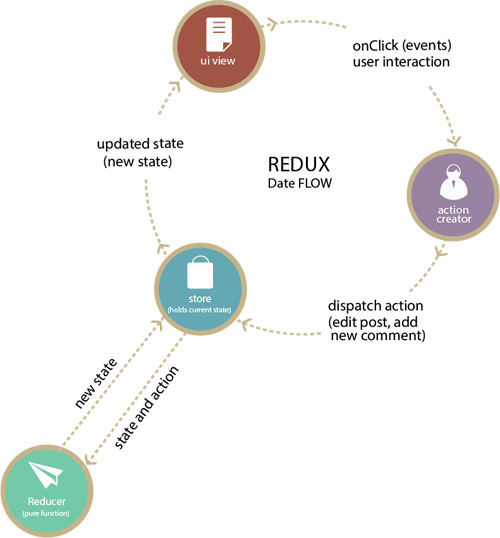
\includegraphics[width=10cm]{image/redux.png}
\caption{Cấu trúc Redux}
\end{figure}
Về cơ bản Redux có 4 thành phần như sau:
\begin{itemize}
    \item Action: Là nơi mang các thông tin dùng để gửi từ ứng dụng đến Store. Các thông tin này là một đối tượng mô tả những gì đã xảy ra.
    \item Reducer: Là nơi xác định State thay đổi như thế nào.
    \item Store: Là nơi quản lý State, cho phép truy cập State qua getState(), update State qua dispatch(action), đăng kí listener qua subscribe(listener).
    \item View: Hiển thị dữ liệu được cung cấp bởi Store
\end{itemize}

Middleware là một lớp nằm giữa ứng dụng và network request, là nơi mà có thể thêm vào CORS headers, logging,... Trong Redux, khái niệm middleware cũng tồn tại và giữ vai trò tương tự, nhưng vấn đề mà middleware trong redux giải quyết thì có điểm khác biệt so với server-side. Trong Redux, middleware là lớp nằm giữa Reducers và Dispatch Actions. Vị trí mà Middleware hoạt động là trước khi Reducers nhận được Actions và sau khi 1 Action được dispatch(). Middleware trong Redux được biết đến nhiều nhất trong việc xử lý ASYNC Action - đó là những Action không sẵn sàng ngay khi 1 Action Creator được gọi tới, thông thường ở đây là các API request.
\begin{figure}[h]
\centering
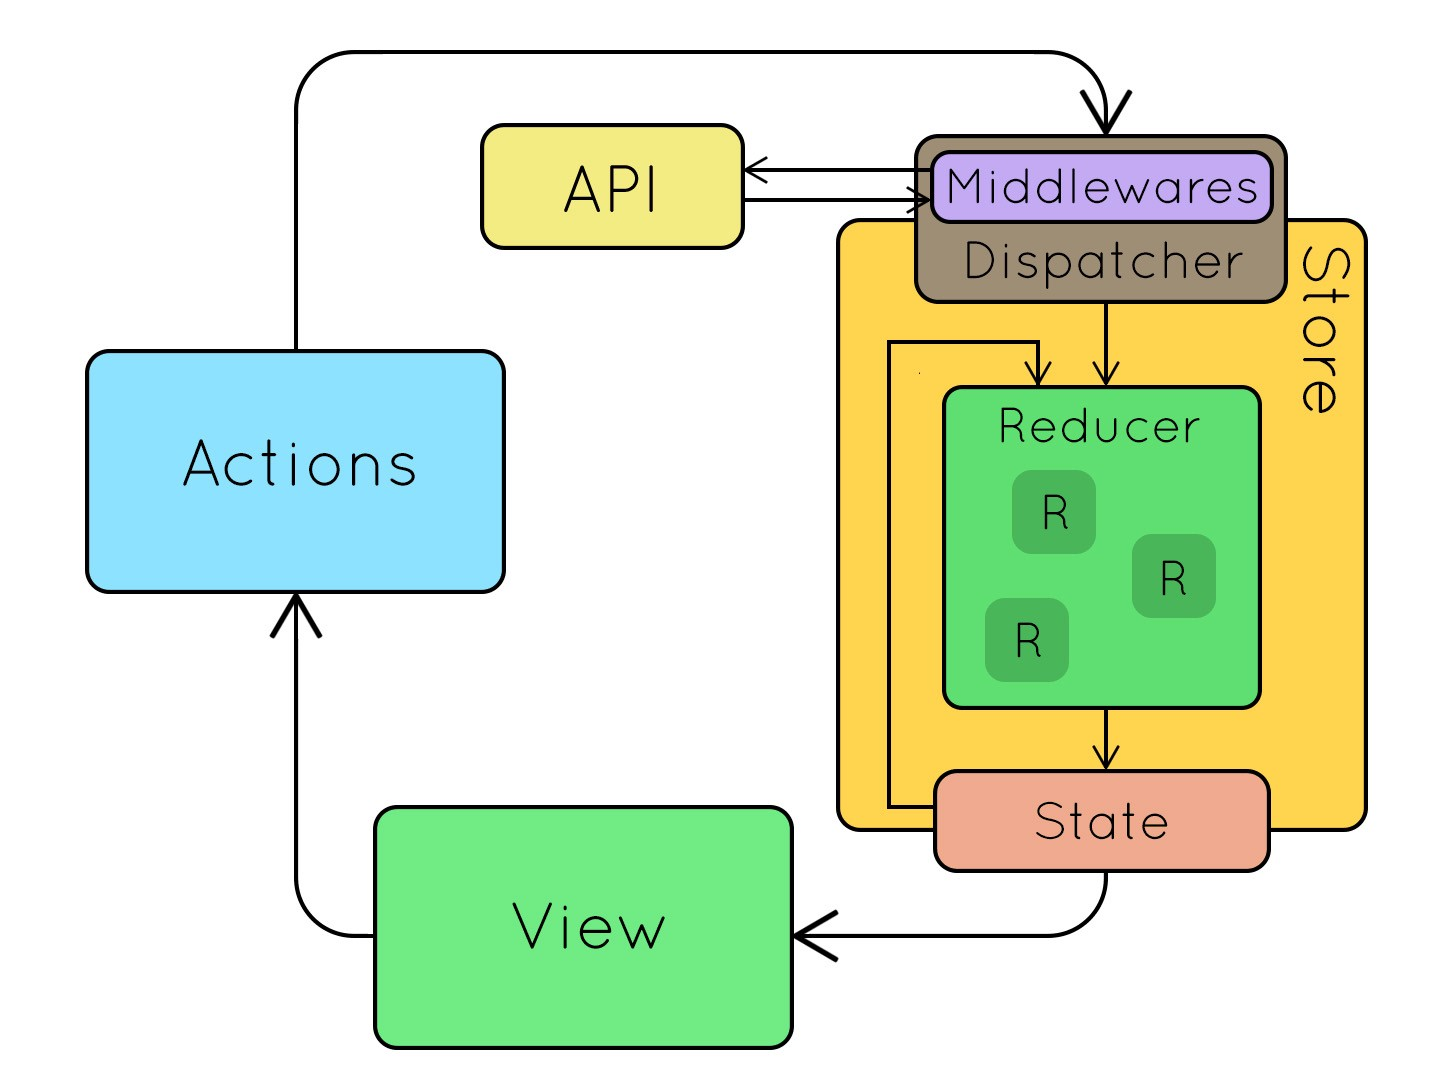
\includegraphics[width=10cm]{image/midleware.jpeg}
\caption{Middleware trong Redux}
\end{figure}
